\section{Lineare Funktionen}\label{sec:Lineare Funktionen}
Wird eine Funktion durch eine Gleichung in der Form $y=mx+b$ dargestellt, so spricht man von einer linearen Funktion. Dabei gibt $b$ den Schnittpunkt mit der $Y$-Achse, den sogenannten $Y$-Achsenabschnitt an. DIe Variable $m$ ist die Steigung der Funktion. Hat $m$ die Form $m=\frac{a}{b}$, so gibt $b$ den Weg auf der $X$-Achse und $a$ den Weg auf der $Y$-Achse an, um von einem Punkt zu dem nächsten zu gelangen. Dies kann gut mit dem Steigungsdreieck darsgestellt werden. Beim Einzeichnen ist zu beachten, dass immer erst nach Rechts und anschließend nach oben bei potiven Zahlen und nach unten bei negativen Zahlen gegangen wird.
\subsection{Parallelität}\label{sec:Lineare Funktionen/Parallelitaet}
 Um die Eigenschaft der Parallelität zu bestimmen bei einer linearen Funktion, betrachtet man den Steigungsfaktor $m$.
Im Bezug auf Parallelität ist folgendes festzuhalten. 
\begin{align*}
	f(x)=mx+b\\
	a(x)=m_1x+b
\end{align*}
Sind die Werte, die $m$ annimmt, die selben, so spricht man von einer Parallelität.
\subsection{Orthogonalität}\label{sec:Lineare Funktionen/Orthogonalitaet}
 Im Vergleich zu der Parallelität stellt die Orthogonalität das Gegenteil dar. Eine Funktion, die zu einer anderen Orthonogal steht, bildet mit der anderen Funktion einen Schnittpunkt im 90\degree Winkel. Daraus folgt, dass sollte $m_f\cdot m_a=-1$ die Funktionen immer orthogonal zu einander stehen.
\begin{figure}[h!]
\centering
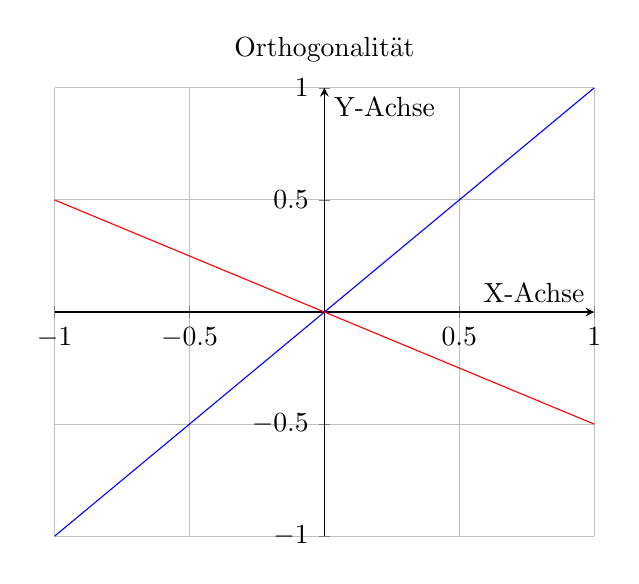
\begin{tikzpicture}
\begin{axis}[
    title={Orthogonalität},
    xlabel={X-Achse},
    ylabel={Y-Achse},
    axis lines=middle, % Zentriert die Achsen
    xmin=-1, xmax=1, % Setzt die Grenzen für die X-Achse
    ymin=-1, ymax=1, % Setzt die Grenzen für die Y-Achse
    grid=major, % Fügt ein Hauptgitter hinzu
]
\addplot+[mark=none] {x};
\addplot+[mark=none] {-(1/2)*x};
\end{axis}
\end{tikzpicture}
\caption{Graphisches Beispiel für Orthogonalität}
\end{figure}
\subsection{Geradengleichung bestimmen}\label{sec:Lineare Funktionen/Geradengleichung}
Bei einer linearen Funktion bei der die Steigung und ein Punkt auf einer Geraden gegeben ist, lässt sich die Funktionsgleichung leicht bestimmen. Hierzu geht man von der Grundform $f(x)=mx+b$ aus und ermittelt $b$ sowie den gesuchten Parameter. Dafür setzt man das Gegebene in die Grundform ein und bestimmt $b$ so, dass die Gleichung erfüllt ist.

\begin{beispiel}
Gesucht ist die Gerade $g_1$ mit $m=3$, die durch den Punkt $(-2;-7)$ verläuft
Dabei wird $g_1:f(x)=mx+b$ wie folgt definiert $m=3$, $x=2$, $y=-7$.
\begin{align*}
	f(x)&=mx+b\\
	-7&=-3\cdot (-2)+b\\
	-7&=6+b\\
	-13&=b
\end{align*}
Somit lautet der $Y$-Achsenabschnitt $(0;-13)$, weswegen die gesuchte Gerade wie folgt lautet: $g_1:f(x)=-3x-13$
\end{beispiel}
\subsection{Zwei-Punkt Steigungsform}\label{sec:Lineare Funktionen/Zwei-Punkt Steigungsform}
Sind von einer Geraden zwei Punkte, der Form $A(y_1;y_2)$ und $B(x_2;y_2)$, bekannt, so kann man aus diesen beiden Punkten ein Steigungsdreieck bilden. Für die Steigung gilt dann folgendes.
\begin{align*}
	m&=\frac{\text{Abstand Y-Wert}}{\text{Abstand X-Wert}}\\
	m&=\frac{y_1-y_2}{x_1-x_2}
\end{align*}

\begin{beispiel}
Die Punkte $A(1,-1)$, $B(2;3)$ sind gegeben und sollen nun mit der Zwei-Punkt Steigungsform die Steigung $m$ ergeben. 
	\begin{align*}
		m&=\frac{y_1-y_2}{x_1-x_2}\\
		m&=\frac{3-(-1)}{2-1}\\
		m&=\frac{4}{1}\\
		m&=4
	\end{align*}
	Somit ist die Steigung $m=4$ zwischen den Punkten $A,B$
\end{beispiel}

